\documentclass[aspectratio=169,11pt]{beamer}

% TEMA Y COLORES
\usetheme{Madrid}
\usecolortheme{whale}

\definecolor{primaryblue}{RGB}{0,102,153}
\definecolor{accentgreen}{RGB}{0,128,0}
\definecolor{accentorange}{RGB}{204,102,0}
\definecolor{darkgray}{RGB}{64,64,64}

\setbeamercolor{palette primary}{bg=primaryblue,fg=white}
\setbeamercolor{palette secondary}{bg=primaryblue!80,fg=white}
\setbeamercolor{palette tertiary}{bg=primaryblue!60,fg=white}
\setbeamercolor{structure}{fg=primaryblue}
\setbeamercolor{block title}{bg=primaryblue,fg=white}
\setbeamercolor{block body}{bg=primaryblue!10}
\setbeamercolor{block title example}{bg=accentgreen,fg=white}
\setbeamercolor{block body example}{bg=accentgreen!10}
\setbeamercolor{block title alerted}{bg=accentorange,fg=white}
\setbeamercolor{block body alerted}{bg=accentorange!10}

% PAQUETES
\usepackage[utf8]{inputenc}
\usepackage[T1]{fontenc}
\usepackage{amsmath,amssymb}
\usepackage{booktabs}
\usepackage{tikz}
\usepackage{pgfplots}
\usepackage{listings}
\usepackage{multicol}

\pgfplotsset{compat=1.17}

% CÓDIGO PYTHON
\lstdefinestyle{pythonstyle}{
    language=Python,
    basicstyle=\ttfamily\footnotesize,
    keywordstyle=\color{blue}\bfseries,
    stringstyle=\color{red},
    commentstyle=\color{accentgreen}\itshape,
    frame=single,
    breaklines=true,
    showstringspaces=false,
    backgroundcolor=\color{gray!10}
}

% NAVEGACIÓN Y PIE DE PÁGINA
\setbeamertemplate{navigation symbols}{}
\setbeamertemplate{footline}{
    \leavevmode%
    \hbox{%
        \begin{beamercolorbox}[wd=.333333\paperwidth,ht=2.25ex,dp=1ex,center]{author in head/foot}%
            \usebeamerfont{author in head/foot}Matemáticas Financieras
        \end{beamercolorbox}%
        \begin{beamercolorbox}[wd=.333333\paperwidth,ht=2.25ex,dp=1ex,center]{title in head/foot}%
            \usebeamerfont{title in head/foot}Sesión 5
        \end{beamercolorbox}%
        \begin{beamercolorbox}[wd=.333333\paperwidth,ht=2.25ex,dp=1ex,right]{date in head/foot}%
            \usebeamerfont{date in head/foot}\insertframenumber{} / \inserttotalframenumber\hspace*{2ex}
        \end{beamercolorbox}}%
    \vskip0pt%
}

\title[Sesión 5]{Anualidades Ordinarias (Vencidas)}
\subtitle{Series de pagos iguales y periódicos}
\author{Matemáticas Financieras}
\institute{Valor del Dinero en el Tiempo}
\date{Semana 3 | Clase 1 | Duración: 1h 50min}

\begin{document}

% ===========================================
% SECCIÓN 1: PORTADA Y CONTENIDO
% ===========================================

\begin{frame}
    \titlepage
\end{frame}

\begin{frame}{Contenido de la Sesión}
    \tableofcontents
\end{frame}

% ===========================================
% SECCIÓN 2: INTRODUCCIÓN
% ===========================================
\section{Introducción}

\begin{frame}{Conexión con las Sesiones Anteriores}
    \begin{block}{Hasta ahora: Flujos Únicos}
        Aprendimos a calcular VP y VF de flujos \textbf{individuales}:
        \[
        F = P(1 + r)^n \quad \text{y} \quad P = \frac{F}{(1 + r)^n}
        \]
    \end{block}

    \pause
    \vspace{0.3cm}

    \begin{alertblock}{Ahora: Flujos Múltiples}
        ¿Qué pasa cuando hay \textbf{múltiples flujos iguales y periódicos}?

        \vspace{0.2cm}
        \textit{Ejemplos: pagos mensuales de un préstamo, depósitos a un fondo de ahorro, rentas, pensiones...}
    \end{alertblock}

    \pause
    \vspace{0.3cm}

    \begin{exampleblock}{Ventaja}
        Existe una fórmula cerrada para calcular VP y VF de estos flujos.
    \end{exampleblock}
\end{frame}

\begin{frame}{Objetivos de Aprendizaje}
    Al finalizar esta sesión, serás capaz de:
    \begin{enumerate}
        \item Identificar y caracterizar una anualidad ordinaria
        \item Derivar la fórmula del valor presente de una anualidad
        \item Derivar la fórmula del valor futuro de una anualidad
        \item Calcular el pago periódico dado VP, VF, tasa y períodos
        \item Aplicar anualidades a fondos de ahorro y préstamos
        \item Usar la HP 12C y Python para cálculos de anualidades
    \end{enumerate}
\end{frame}

\begin{frame}{Motivación: El Problema del Préstamo}
    \begin{block}{Escenario Común}
        Pides un préstamo de \$500,000 para comprar un auto.
        \begin{itemize}
            \item Tasa: 12\% anual (1\% mensual)
            \item Plazo: 48 meses
            \item Pagos mensuales iguales
        \end{itemize}

        ¿Cuánto será tu pago mensual?
    \end{block}

    \pause
    \vspace{0.3cm}

    \textbf{Sin fórmula de anualidades:}
    \begin{itemize}
        \item Tendríamos que plantear 48 ecuaciones
        \item O usar métodos de prueba y error
    \end{itemize}

    \pause
    \vspace{0.3cm}

    \textbf{Con fórmula de anualidades:}
    \begin{itemize}
        \item Un solo cálculo directo
        \item Respuesta: \$13,166.75 mensuales
    \end{itemize}
\end{frame}

\begin{frame}{¿Qué es una Anualidad?}
    \begin{block}{Definición}
        Una \textbf{anualidad} es una serie de pagos iguales ($PMT$) realizados a intervalos regulares de tiempo durante un período determinado.
    \end{block}

    \pause
    \vspace{0.3cm}

    \textbf{Características:}
    \begin{enumerate}
        \item Pagos de \textbf{monto igual}
        \item Pagos a \textbf{intervalos regulares} (mes, trimestre, año)
        \item \textbf{Tasa de interés constante} durante todo el período
        \item Número \textbf{finito} de pagos
    \end{enumerate}

    \pause
    \vspace{0.3cm}

    \begin{alertblock}{Nota sobre el nombre}
        A pesar de llamarse ``anualidad'', los pagos no tienen que ser anuales. El nombre viene de la palabra latina ``annus'' (año), pero aplica a cualquier período.
    \end{alertblock}
\end{frame}

\begin{frame}{Tipos de Anualidades}
    \begin{columns}
        \begin{column}{0.48\textwidth}
            \begin{block}{Anualidad Ordinaria (Vencida)}
                Pagos al \textbf{final} de cada período.

                \vspace{0.3cm}
                \textbf{Ejemplos:}
                \begin{itemize}
                    \item Pagos de préstamos
                    \item Cupones de bonos
                    \item Salarios
                \end{itemize}
            \end{block}
        \end{column}

        \begin{column}{0.48\textwidth}
            \begin{block}{Anualidad Anticipada}
                Pagos al \textbf{inicio} de cada período.

                \vspace{0.3cm}
                \textbf{Ejemplos:}
                \begin{itemize}
                    \item Rentas (alquileres)
                    \item Primas de seguros
                    \item Cuotas de membresía
                \end{itemize}
            \end{block}
        \end{column}
    \end{columns}

    \pause
    \vspace{0.5cm}

    \begin{center}
        \textbf{Hoy nos enfocamos en anualidades ordinarias (vencidas).}

        Las anticipadas se verán en la Sesión 6.
    \end{center}
\end{frame}

% ===========================================
% SECCIÓN 3: DERIVACIONES MATEMÁTICAS
% ===========================================
\section{Valor Presente de una Anualidad}

\begin{frame}{Diagrama de una Anualidad Ordinaria}
    \begin{center}
        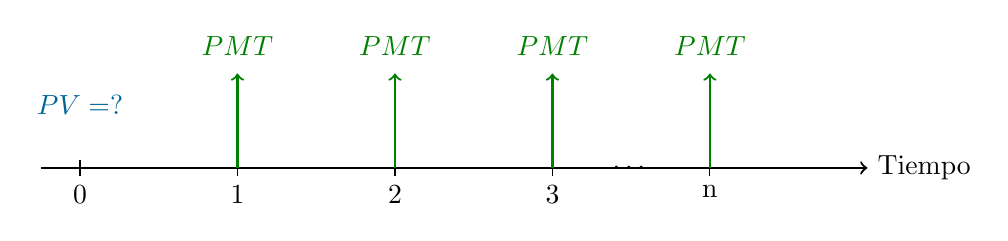
\begin{tikzpicture}[scale=1.0]
            % Línea de tiempo
            \draw[thick, ->] (-0.5,0) -- (10,0) node[right] {Tiempo};

            % Marcas de tiempo
            \foreach \x/\label in {0/0, 2/1, 4/2, 6/3, 8/n} {
                \draw (\x,0.1) -- (\x,-0.1) node[below] {\label};
            }

            % Puntos suspensivos
            \node at (7,0) {$\cdots$};

            % Pagos (al final de cada período)
            \foreach \x in {2, 4, 6, 8} {
                \draw[thick, ->, accentgreen] (\x,0) -- (\x,1.2);
            }

            % Etiquetas PMT
            \node[accentgreen, above] at (2,1.3) {$PMT$};
            \node[accentgreen, above] at (4,1.3) {$PMT$};
            \node[accentgreen, above] at (6,1.3) {$PMT$};
            \node[accentgreen, above] at (8,1.3) {$PMT$};

            % VP
            \node[primaryblue] at (0,0.8) {$PV = ?$};
        \end{tikzpicture}
    \end{center}

    \pause
    \vspace{0.3cm}

    \textbf{Observaciones clave:}
    \begin{itemize}
        \item El primer pago ocurre al final del período 1 (no en $t=0$)
        \item Hay $n$ pagos en total
        \item Queremos encontrar el VP en $t=0$
    \end{itemize}
\end{frame}

\begin{frame}{Derivación del VP: Método de Suma}
    El VP es la suma de los VP de cada pago individual:

    \pause
    \begin{align*}
        PV &= \frac{PMT}{(1+r)^1} + \frac{PMT}{(1+r)^2} + \frac{PMT}{(1+r)^3} + \cdots + \frac{PMT}{(1+r)^n}
    \end{align*}

    \pause
    Factorizando $PMT$:
    \begin{align*}
        PV &= PMT \left[ \frac{1}{(1+r)^1} + \frac{1}{(1+r)^2} + \cdots + \frac{1}{(1+r)^n} \right]
    \end{align*}

    \pause
    El corchete es una \textbf{serie geométrica} con:
    \begin{itemize}
        \item Primer término: $a = \frac{1}{1+r}$
        \item Razón común: $q = \frac{1}{1+r}$
        \item $n$ términos
    \end{itemize}
\end{frame}

\begin{frame}{Derivación del VP: Fórmula de Serie Geométrica}
    La suma de una serie geométrica es:
    \[
    S_n = a \cdot \frac{1 - q^n}{1 - q}
    \]

    \pause
    Sustituyendo $a = \frac{1}{1+r}$ y $q = \frac{1}{1+r}$:
    \begin{align*}
        S_n &= \frac{1}{1+r} \cdot \frac{1 - \left(\frac{1}{1+r}\right)^n}{1 - \frac{1}{1+r}}
    \end{align*}

    \pause
    Simplificando el denominador: $1 - \frac{1}{1+r} = \frac{r}{1+r}$
    \begin{align*}
        S_n &= \frac{1}{1+r} \cdot \frac{1 - (1+r)^{-n}}{\frac{r}{1+r}} = \frac{1 - (1+r)^{-n}}{r}
    \end{align*}
\end{frame}

\begin{frame}{Fórmula del Valor Presente de una Anualidad}
    \begin{block}{Valor Presente de una Anualidad Ordinaria}
        \[
        \boxed{PV = PMT \cdot \frac{1 - (1+r)^{-n}}{r}}
        \]
    \end{block}

    \pause
    \vspace{0.3cm}

    \begin{block}{Factor de Valor Presente de Anualidad (PVIFA)}
        \[
        \boxed{PVIFA_{r,n} = \frac{1 - (1+r)^{-n}}{r}}
        \]
        Por lo tanto: $PV = PMT \cdot PVIFA_{r,n}$
    \end{block}

    \pause
    \vspace{0.3cm}

    \begin{exampleblock}{Interpretación}
        El PVIFA indica cuántos pesos de hoy equivale recibir \$1 al final de cada uno de los próximos $n$ períodos, dado una tasa $r$.
    \end{exampleblock}
\end{frame}

\section{Valor Futuro de una Anualidad}

\begin{frame}{Diagrama del Valor Futuro}
    \begin{center}
        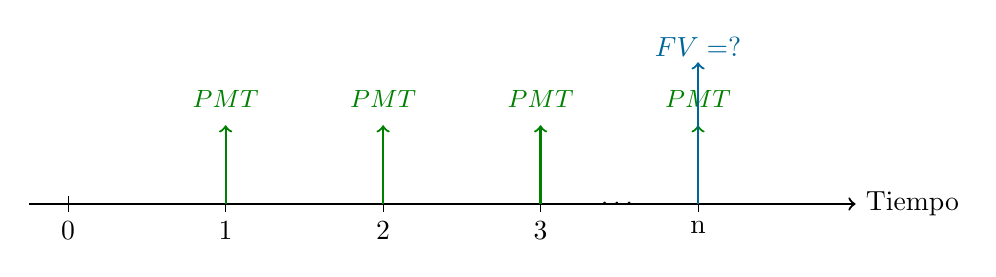
\begin{tikzpicture}[scale=1.0]
            % Línea de tiempo
            \draw[thick, ->] (-0.5,0) -- (10,0) node[right] {Tiempo};

            % Marcas de tiempo
            \foreach \x/\label in {0/0, 2/1, 4/2, 6/3, 8/n} {
                \draw (\x,0.1) -- (\x,-0.1) node[below] {\label};
            }

            % Puntos suspensivos
            \node at (7,0) {$\cdots$};

            % Pagos
            \foreach \x in {2, 4, 6, 8} {
                \draw[thick, ->, accentgreen] (\x,0) -- (\x,1.0);
            }

            % Etiquetas PMT
            \node[accentgreen, above] at (2,1.1) {\small $PMT$};
            \node[accentgreen, above] at (4,1.1) {\small $PMT$};
            \node[accentgreen, above] at (6,1.1) {\small $PMT$};
            \node[accentgreen, above] at (8,1.1) {\small $PMT$};

            % FV
            \node[primaryblue] at (8,2) {$FV = ?$};
            \draw[thick, ->, primaryblue] (8,0) -- (8,1.8);
        \end{tikzpicture}
    \end{center}

    \pause
    \vspace{0.3cm}

    \textbf{Pregunta:} ¿Cuánto tendremos acumulado en $t = n$ si depositamos $PMT$ al final de cada período?
\end{frame}

\begin{frame}{Derivación del VF: Método de Suma}
    Cada pago crece a diferente tasa:

    \pause
    \begin{align*}
        FV &= PMT(1+r)^{n-1} + PMT(1+r)^{n-2} + \cdots + PMT(1+r)^1 + PMT
    \end{align*}

    \pause
    El primer pago (en $t=1$) crece por $n-1$ períodos.

    El último pago (en $t=n$) no gana interés (acaba de llegar).

    \pause
    \vspace{0.3cm}

    Factorizando:
    \begin{align*}
        FV &= PMT \left[ (1+r)^{n-1} + (1+r)^{n-2} + \cdots + (1+r) + 1 \right]
    \end{align*}

    \pause
    Otra serie geométrica con:
    \begin{itemize}
        \item $a = 1$, $q = (1+r)$, $n$ términos
    \end{itemize}
\end{frame}

\begin{frame}{Fórmula del Valor Futuro de una Anualidad}
    Usando la fórmula de serie geométrica con $a=1$ y $q = (1+r)$:
    \begin{align*}
        S_n = \frac{(1+r)^n - 1}{(1+r) - 1} = \frac{(1+r)^n - 1}{r}
    \end{align*}

    \pause
    \vspace{0.3cm}

    \begin{block}{Valor Futuro de una Anualidad Ordinaria}
        \[
        \boxed{FV = PMT \cdot \frac{(1+r)^n - 1}{r}}
        \]
    \end{block}

    \pause

    \begin{block}{Factor de Valor Futuro de Anualidad (FVIFA)}
        \[
        \boxed{FVIFA_{r,n} = \frac{(1+r)^n - 1}{r}}
        \]
        Por lo tanto: $FV = PMT \cdot FVIFA_{r,n}$
    \end{block}
\end{frame}

\begin{frame}{Relación entre PVIFA y FVIFA}
    \begin{alertblock}{Relación Importante}
        \[
        \boxed{FV = PV \cdot (1+r)^n}
        \]

        Por lo tanto:
        \[
        FVIFA_{r,n} = PVIFA_{r,n} \cdot (1+r)^n
        \]
    \end{alertblock}

    \pause
    \vspace{0.3cm}

    \textbf{Verificación:}
    \begin{align*}
        PVIFA \cdot (1+r)^n &= \frac{1 - (1+r)^{-n}}{r} \cdot (1+r)^n \\
        &= \frac{(1+r)^n - 1}{r} = FVIFA \quad \checkmark
    \end{align*}
\end{frame}

\section{Despejando el Pago (PMT)}

\begin{frame}{Cálculo del Pago Periódico}
    A menudo necesitamos encontrar $PMT$ dado $PV$ o $FV$.

    \pause
    \vspace{0.3cm}

    \textbf{Dado el Valor Presente:}
    \begin{align*}
        PV &= PMT \cdot \frac{1 - (1+r)^{-n}}{r}
    \end{align*}

    \begin{block}{Pago dado VP}
        \[
        \boxed{PMT = PV \cdot \frac{r}{1 - (1+r)^{-n}}}
        \]
    \end{block}

    \pause
    \textbf{Dado el Valor Futuro:}
    \begin{block}{Pago dado VF}
        \[
        \boxed{PMT = FV \cdot \frac{r}{(1+r)^n - 1}}
        \]
    \end{block}
\end{frame}

% ===========================================
% SECCIÓN 4: INTERPRETACIÓN VISUAL
% ===========================================
\section{Interpretación Visual}

\begin{frame}{Visualización del VP de una Anualidad}
    \begin{center}
        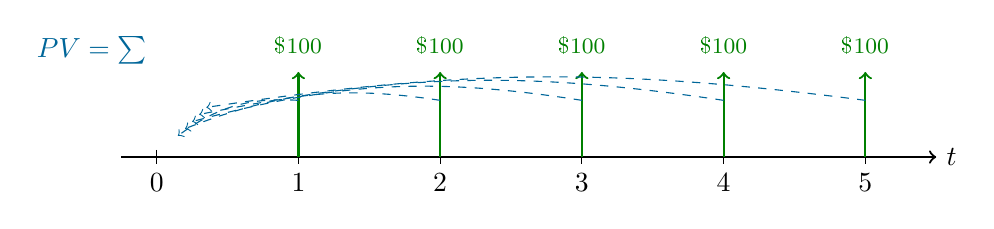
\begin{tikzpicture}[scale=0.9]
            % Línea de tiempo
            \draw[thick, ->] (-0.5,0) -- (11,0) node[right] {$t$};

            % Marcas
            \foreach \x/\label in {0/0, 2/1, 4/2, 6/3, 8/4, 10/5} {
                \draw (\x,0.1) -- (\x,-0.1) node[below] {\label};
            }

            % Pagos
            \foreach \x in {2, 4, 6, 8, 10} {
                \draw[thick, ->, accentgreen] (\x,0) -- (\x,1.2);
                \node[accentgreen, above] at (\x,1.3) {\footnotesize \$100};
            }

            % Flechas de descuento
            \draw[->, primaryblue, dashed] (2,0.8) to[bend right=20] (0.3,0.3);
            \draw[->, primaryblue, dashed] (4,0.8) to[bend right=15] (0.4,0.4);
            \draw[->, primaryblue, dashed] (6,0.8) to[bend right=12] (0.5,0.5);
            \draw[->, primaryblue, dashed] (8,0.8) to[bend right=10] (0.6,0.6);
            \draw[->, primaryblue, dashed] (10,0.8) to[bend right=8] (0.7,0.7);

            % VP total
            \node[primaryblue, left] at (0,1.5) {$PV = \sum$};
        \end{tikzpicture}
    \end{center}

    \pause
    \vspace{0.3cm}

    \textbf{Ejemplo:} 5 pagos de \$100 al 10\%

    $PV = 100 \cdot \frac{1-(1.10)^{-5}}{0.10} = 100 \times 3.7908 = \$379.08$
\end{frame}

\begin{frame}{PVIFA para Diferentes Tasas y Plazos}
    \begin{center}
        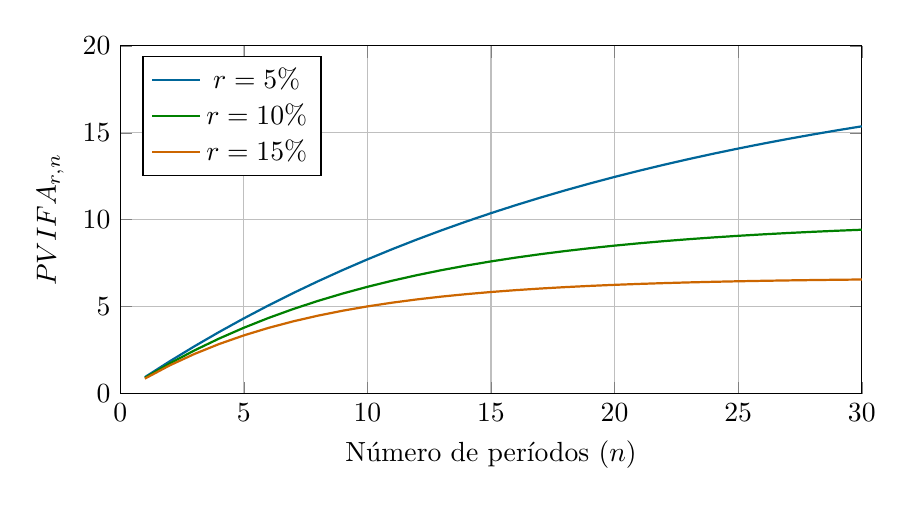
\begin{tikzpicture}
            \begin{axis}[
                xlabel={Número de períodos ($n$)},
                ylabel={$PVIFA_{r,n}$},
                xmin=0, xmax=30,
                ymin=0, ymax=20,
                grid=major,
                width=11cm,
                height=6cm,
                legend pos=north west
            ]
            \addplot[color=primaryblue, thick, domain=1:30, samples=30] {(1-(1.05)^(-x))/0.05};
            \addlegendentry{$r = 5\%$}
            \addplot[color=accentgreen, thick, domain=1:30, samples=30] {(1-(1.10)^(-x))/0.10};
            \addlegendentry{$r = 10\%$}
            \addplot[color=accentorange, thick, domain=1:30, samples=30] {(1-(1.15)^(-x))/0.15};
            \addlegendentry{$r = 15\%$}
            \end{axis}
        \end{tikzpicture}
    \end{center}

    A menor tasa, mayor PVIFA (los flujos futuros valen más hoy).
\end{frame}

\begin{frame}{Visualización del VF de una Anualidad}
    \begin{center}
        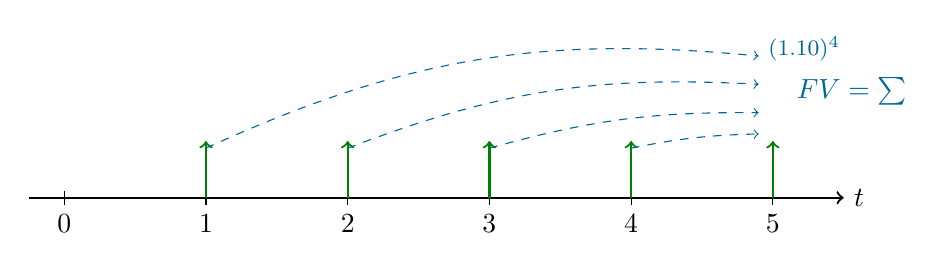
\begin{tikzpicture}[scale=0.9]
            % Línea de tiempo
            \draw[thick, ->] (-0.5,0) -- (11,0) node[right] {$t$};

            % Marcas
            \foreach \x/\label in {0/0, 2/1, 4/2, 6/3, 8/4, 10/5} {
                \draw (\x,0.1) -- (\x,-0.1) node[below] {\label};
            }

            % Pagos y su crecimiento
            \draw[thick, ->, accentgreen] (2,0) -- (2,0.8);
            \draw[->, primaryblue, dashed] (2,0.7) to[bend left=15] (9.8,2.0);
            \node[primaryblue, right] at (9.8,2.1) {\footnotesize $(1.10)^4$};

            \draw[thick, ->, accentgreen] (4,0) -- (4,0.8);
            \draw[->, primaryblue, dashed] (4,0.7) to[bend left=12] (9.8,1.6);

            \draw[thick, ->, accentgreen] (6,0) -- (6,0.8);
            \draw[->, primaryblue, dashed] (6,0.7) to[bend left=8] (9.8,1.2);

            \draw[thick, ->, accentgreen] (8,0) -- (8,0.8);
            \draw[->, primaryblue, dashed] (8,0.7) to[bend left=5] (9.8,0.9);

            \draw[thick, ->, accentgreen] (10,0) -- (10,0.8);

            % FV total
            \node[primaryblue, right] at (10.2,1.5) {$FV = \sum$};
        \end{tikzpicture}
    \end{center}

    \textbf{Ejemplo:} 5 depósitos de \$100 al 10\%

    $FV = 100 \cdot \frac{(1.10)^5 - 1}{0.10} = 100 \times 6.1051 = \$610.51$
\end{frame}

% ===========================================
% SECCIÓN 5: TRUCOS DE ESTIMACIÓN
% ===========================================
\section{Trucos de Estimación Mental}

\begin{frame}{Aproximación para el PVIFA}
    \begin{alertblock}{Para tasas bajas y plazos largos}
        Cuando $n$ es grande, $(1+r)^{-n} \to 0$, entonces:
        \[
        PVIFA_{r,n} \approx \frac{1}{r}
        \]
        Este es el valor de una \textbf{perpetuidad} (la veremos en la sesión 6).
    \end{alertblock}

    \pause
    \vspace{0.3cm}

    \textbf{Ejemplo:} PVIFA al 5\% por 50 años

    Aproximación: $1/0.05 = 20$

    Exacto: $\frac{1-(1.05)^{-50}}{0.05} = 18.26$

    \pause
    \vspace{0.3cm}

    \begin{exampleblock}{Uso práctico}
        Si alguien dice ``Esta inversión paga \$1,000 anuales por 30 años al 5\%'', puedes estimar rápidamente: VP $\approx$ \$20,000 (en realidad \$15,372).
    \end{exampleblock}
\end{frame}

\begin{frame}{Tabla de PVIFA}
    \textbf{Factor de Valor Presente de Anualidad:}

    \vspace{0.3cm}

    \begin{center}
    \begin{tabular}{@{}c|ccccc@{}}
        \toprule
        $r$ \textbackslash{} $n$ & 5 & 10 & 15 & 20 & 30 \\
        \midrule
        5\% & 4.33 & 7.72 & 10.38 & 12.46 & 15.37 \\
        8\% & 3.99 & 6.71 & 8.56 & 9.82 & 11.26 \\
        10\% & 3.79 & 6.14 & 7.61 & 8.51 & 9.43 \\
        12\% & 3.60 & 5.65 & 6.81 & 7.47 & 8.06 \\
        15\% & 3.35 & 5.02 & 5.85 & 6.26 & 6.57 \\
        \bottomrule
    \end{tabular}
    \end{center}

    \pause
    \vspace{0.3cm}

    \begin{exampleblock}{Uso}
        VP de 20 pagos de \$5,000 al 10\%:

        $PV = 5,000 \times 8.51 = \$42,550$
    \end{exampleblock}
\end{frame}

\begin{frame}{El ``Factor de Recuperación de Capital''}
    \begin{alertblock}{Definición}
        El inverso del PVIFA indica cuánto pago anual se necesita para ``recuperar'' (o amortizar) \$1 de deuda:
        \[
        \text{FRC} = \frac{r}{1-(1+r)^{-n}} = \frac{1}{PVIFA}
        \]
    \end{alertblock}

    \pause
    \vspace{0.3cm}

    \textbf{Ejemplo:} ¿Pago mensual de un préstamo de \$100,000 a 5 años al 12\% anual (1\% mensual)?

    $n = 60$ meses, $r = 1\%$

    \pause
    $PVIFA = \frac{1-(1.01)^{-60}}{0.01} = 44.955$

    $PMT = 100,000 / 44.955 = \$2,224.44$ mensuales
\end{frame}

% ===========================================
% SECCIÓN 6: HP 12C
% ===========================================
\section{Calculadora HP 12C}

\begin{frame}{HP 12C: Teclas para Anualidades}
    \begin{center}
    \begin{tabular}{@{}cl@{}}
        \toprule
        \textbf{Tecla} & \textbf{Función} \\
        \midrule
        \texttt{n} & Número de períodos (pagos) \\
        \texttt{i} & Tasa de interés por período (\%) \\
        \texttt{PV} & Valor presente \\
        \texttt{PMT} & Pago periódico \\
        \texttt{FV} & Valor futuro \\
        \texttt{g END} & Modo anualidad ordinaria (default) \\
        \texttt{g BEG} & Modo anualidad anticipada \\
        \bottomrule
    \end{tabular}
    \end{center}

    \pause
    \vspace{0.3cm}

    \begin{alertblock}{Convención de Signos}
        \begin{itemize}
            \item Flujos que \textbf{salen} de ti: negativos
            \item Flujos que \textbf{entran} a ti: positivos
            \item PV y FV deben tener signos opuestos a PMT (o uno de ellos ser 0)
        \end{itemize}
    \end{alertblock}
\end{frame}

\begin{frame}{HP 12C: Ejemplo 1 - Calcular Pago de Préstamo}
    \begin{block}{Problema}
        Préstamo de \$500,000, 48 meses, 1\% mensual. ¿Cuál es el pago mensual?
    \end{block}

    \pause
    \vspace{0.3cm}

    \begin{center}
    \begin{tabular}{@{}lll@{}}
        \toprule
        \textbf{Teclas} & \textbf{Display} & \textbf{Descripción} \\
        \midrule
        \texttt{f CLX} & 0.00 & Limpiar \\
        \texttt{g END} & & Modo ordinario \\
        \texttt{500000 PV} & 500,000.00 & Préstamo recibido (+) \\
        \texttt{48 n} & 48.00 & 48 meses \\
        \texttt{1 i} & 1.00 & 1\% mensual \\
        \texttt{0 FV} & 0.00 & Sin valor residual \\
        \texttt{PMT} & \textbf{-13,166.75} & Pago mensual \\
        \bottomrule
    \end{tabular}
    \end{center}

    \pause
    \textbf{Respuesta:} \$13,166.75 mensuales (negativo porque sale de ti).
\end{frame}

\begin{frame}{HP 12C: Ejemplo 2 - Calcular VP de Anualidad}
    \begin{block}{Problema}
        Una inversión paga \$10,000 anuales por 15 años. Si la tasa es 8\%, ¿cuánto vale hoy?
    \end{block}

    \pause
    \vspace{0.3cm}

    \begin{center}
    \begin{tabular}{@{}lll@{}}
        \toprule
        \textbf{Teclas} & \textbf{Display} & \textbf{Descripción} \\
        \midrule
        \texttt{f CLX} & 0.00 & Limpiar \\
        \texttt{g END} & & Modo ordinario \\
        \texttt{10000 PMT} & 10,000.00 & Pago que recibes (+) \\
        \texttt{15 n} & 15.00 & 15 años \\
        \texttt{8 i} & 8.00 & 8\% anual \\
        \texttt{0 FV} & 0.00 & Sin valor final \\
        \texttt{PV} & \textbf{-85,594.79} & Valor presente \\
        \bottomrule
    \end{tabular}
    \end{center}

    \pause
    \textbf{Respuesta:} \$85,594.79 (negativo indica cuánto pagarías hoy).
\end{frame}

\begin{frame}{HP 12C: Ejemplo 3 - Fondo de Ahorro}
    \begin{block}{Problema}
        Quieres ahorrar \$1,000,000 en 20 años. Si el fondo paga 6\% anual, ¿cuánto debes depositar cada año?
    \end{block}

    \pause
    \vspace{0.3cm}

    \begin{center}
    \begin{tabular}{@{}lll@{}}
        \toprule
        \textbf{Teclas} & \textbf{Display} & \textbf{Descripción} \\
        \midrule
        \texttt{f CLX} & 0.00 & Limpiar \\
        \texttt{g END} & & Modo ordinario \\
        \texttt{1000000 FV} & 1,000,000.00 & Meta de ahorro (+) \\
        \texttt{20 n} & 20.00 & 20 años \\
        \texttt{6 i} & 6.00 & 6\% anual \\
        \texttt{0 PV} & 0.00 & Sin inversión inicial \\
        \texttt{PMT} & \textbf{-27,184.56} & Depósito anual \\
        \bottomrule
    \end{tabular}
    \end{center}

    \pause
    \textbf{Respuesta:} Debes depositar \$27,184.56 anuales.
\end{frame}

% ===========================================
% SECCIÓN 7: EJERCICIOS PRÁCTICOS
% ===========================================
\section{Ejercicios Prácticos}

\begin{frame}{Ejercicio 1: Préstamo de Auto}
    \begin{block}{Problema}
        Financias un auto de \$350,000 a 36 meses con tasa del 18\% anual (1.5\% mensual). ¿Cuál es el pago mensual?
    \end{block}

    \pause
    \vspace{0.3cm}

    \textbf{Solución:}
    \begin{align*}
        PMT &= PV \cdot \frac{r}{1-(1+r)^{-n}} \\[0.2cm]
        PMT &= 350,000 \cdot \frac{0.015}{1-(1.015)^{-36}} \\[0.2cm]
        PMT &= 350,000 \cdot \frac{0.015}{1-0.5851} \\[0.2cm]
        PMT &= 350,000 \cdot \frac{0.015}{0.4149} \\[0.2cm]
        PMT &= 350,000 \cdot 0.03615 = \$12,652.68
    \end{align*}
\end{frame}

\begin{frame}{Ejercicio 2: Valor de una Anualidad}
    \begin{block}{Problema}
        Una renta vitalicia paga \$25,000 anuales por 30 años, comenzando en un año. Si la tasa de descuento es 7\%, ¿cuánto vale hoy?
    \end{block}

    \pause
    \vspace{0.3cm}

    \textbf{Solución:}
    \begin{align*}
        PV &= PMT \cdot \frac{1-(1+r)^{-n}}{r} \\[0.2cm]
        PV &= 25,000 \cdot \frac{1-(1.07)^{-30}}{0.07} \\[0.2cm]
        PV &= 25,000 \cdot \frac{1-0.1314}{0.07} \\[0.2cm]
        PV &= 25,000 \cdot 12.409 = \$310,225
    \end{align*}
\end{frame}

\begin{frame}{Ejercicio 3: Fondo de Retiro}
    \begin{block}{Problema}
        Quieres tener \$5,000,000 al retirarte en 30 años. Si tu fondo rinde 8\% anual, ¿cuánto debes aportar mensualmente? (Usa tasa mensual equivalente)
    \end{block}

    \pause
    \vspace{0.2cm}

    \textbf{Tasa mensual:} $r_m = (1.08)^{1/12} - 1 = 0.6434\%$

    \textbf{Períodos:} $n = 30 \times 12 = 360$

    \pause
    \textbf{Solución:}
    \begin{align*}
        PMT &= FV \cdot \frac{r}{(1+r)^n - 1} \\[0.2cm]
        PMT &= 5,000,000 \cdot \frac{0.006434}{(1.006434)^{360} - 1} \\[0.2cm]
        PMT &= 5,000,000 \cdot \frac{0.006434}{9.0627} \\[0.2cm]
        PMT &= \$3,549.04 \text{ mensuales}
    \end{align*}
\end{frame}

\begin{frame}{Ejercicio 4: ¿Cuántos Pagos?}
    \begin{block}{Problema}
        Tienes una deuda de \$80,000 que pagas con mensualidades de \$2,500 al 1.5\% mensual. ¿En cuántos meses la pagas?
    \end{block}

    \pause
    \vspace{0.3cm}

    \textbf{Solución:}
    \begin{align*}
        PV &= PMT \cdot \frac{1-(1+r)^{-n}}{r} \\
        80,000 &= 2,500 \cdot \frac{1-(1.015)^{-n}}{0.015} \\
        \frac{80,000 \times 0.015}{2,500} &= 1 - (1.015)^{-n} \\
        0.48 &= 1 - (1.015)^{-n} \\
        (1.015)^{-n} &= 0.52 \\
        -n \cdot \ln(1.015) &= \ln(0.52) \\
        n &= \frac{-\ln(0.52)}{\ln(1.015)} = \frac{0.6539}{0.0149} = 43.9 \approx 44 \text{ meses}
    \end{align*}
\end{frame}

\begin{frame}{Ejercicio 5: Comparación de Préstamos}
    \begin{block}{Problema}
        Banco A: \$200,000 a 24 meses, 1.2\% mensual.

        Banco B: \$200,000 a 36 meses, 1.0\% mensual.

        ¿Cuál tiene menor pago? ¿Cuál paga menos intereses totales?
    \end{block}

    \pause
    \vspace{0.2cm}

    \textbf{Banco A:}
    $PMT_A = 200,000 \cdot \frac{0.012}{1-(1.012)^{-24}} = \$9,526.67$

    Total pagado: $9,526.67 \times 24 = \$228,640$

    Intereses: $228,640 - 200,000 = \$28,640$

    \pause

    \textbf{Banco B:}
    $PMT_B = 200,000 \cdot \frac{0.01}{1-(1.01)^{-36}} = \$6,643.38$

    Total pagado: $6,643.38 \times 36 = \$239,162$

    Intereses: $239,162 - 200,000 = \$39,162$

    \pause
    \textbf{Banco B} tiene menor pago, pero \textbf{Banco A} paga menos intereses totales.
\end{frame}

% ===========================================
% SECCIÓN 8: PYTHON
% ===========================================
\section{Python con numpy-financial}

\begin{frame}[fragile]{Python: Funciones de Anualidades}
    \begin{lstlisting}[style=pythonstyle]
import numpy_financial as npf

# Calcular pago de prestamo
pv = 500000      # Monto del prestamo
n = 48           # Meses
r = 0.01         # 1% mensual

pmt = npf.pmt(rate=r, nper=n, pv=pv, fv=0)
print(f"Pago mensual: ${-pmt:,.2f}")

# Calcular valor presente de anualidad
pmt_anual = 10000
n_años = 15
r_anual = 0.08

pv = npf.pv(rate=r_anual, nper=n_años, pmt=pmt_anual, fv=0)
print(f"Valor presente: ${-pv:,.2f}")

# Calcular valor futuro (fondo de ahorro)
aporte = -5000   # Deposito mensual
n = 240          # 20 años en meses
r = 0.005        # 0.5% mensual

fv = npf.fv(rate=r, nper=n, pmt=aporte, pv=0)
print(f"Valor futuro: ${fv:,.2f}")
    \end{lstlisting}
\end{frame}

\begin{frame}[fragile]{Python: Tabla de Amortización (Preview)}
    \begin{lstlisting}[style=pythonstyle]
import numpy_financial as npf

def tabla_amortizacion(pv, r, n):
    pmt = -npf.pmt(r, n, pv)
    saldo = pv

    print("Mes | Pago     | Interes  | Capital  | Saldo")
    print("-" * 55)

    for mes in range(1, min(n+1, 6)):  # Primeros 5 meses
        interes = saldo * r
        capital = pmt - interes
        saldo -= capital
        print(f"{mes:3d} | ${pmt:8,.2f} | ${interes:8,.2f} | ${capital:8,.2f} | ${saldo:10,.2f}")

    print("...")

# Ejemplo
tabla_amortizacion(100000, 0.01, 36)
    \end{lstlisting}

    \textbf{Nota:} La tabla completa de amortización se verá en la Sesión 7.
\end{frame}

\begin{frame}[fragile]{Python: Comparación de Escenarios}
    \begin{lstlisting}[style=pythonstyle]
import numpy_financial as npf
import matplotlib.pyplot as plt
import numpy as np

# Comparar crecimiento de fondo de ahorro
aporte_mensual = 1000
años = 30
meses = np.arange(1, años*12 + 1)

tasas = [0.005, 0.007, 0.01]  # 6%, 8.4%, 12% anual aprox
labels = ['6%', '8.4%', '12%']

plt.figure(figsize=(10, 6))
for r, label in zip(tasas, labels):
    fv = [-npf.fv(r, m, -aporte_mensual, 0) for m in meses]
    plt.plot(meses/12, np.array(fv)/1000, label=f'Tasa {label} anual')

plt.xlabel('Años')
plt.ylabel('Valor acumulado (miles $)')
plt.title('Crecimiento de Fondo de Ahorro')
plt.legend()
plt.grid(True)
    \end{lstlisting}
\end{frame}

% ===========================================
% SECCIÓN 9: RESUMEN Y TAREA
% ===========================================
\section{Resumen y Tarea}

\begin{frame}{Resumen de Fórmulas}
    \begin{columns}
        \begin{column}{0.5\textwidth}
            \textbf{Valor Presente}
            \[
            PV = PMT \cdot \frac{1-(1+r)^{-n}}{r}
            \]

            \textbf{Pago dado VP}
            \[
            PMT = PV \cdot \frac{r}{1-(1+r)^{-n}}
            \]
        \end{column}

        \begin{column}{0.5\textwidth}
            \textbf{Valor Futuro}
            \[
            FV = PMT \cdot \frac{(1+r)^n - 1}{r}
            \]

            \textbf{Pago dado VF}
            \[
            PMT = FV \cdot \frac{r}{(1+r)^n - 1}
            \]
        \end{column}
    \end{columns}

    \vspace{0.5cm}

    \textbf{Relación:} $FV = PV \cdot (1+r)^n$
\end{frame}

\begin{frame}{Conceptos Clave}
    \begin{enumerate}
        \item Una \textbf{anualidad} es una serie de pagos iguales y periódicos
        \item \textbf{Anualidad ordinaria}: pagos al final de cada período
        \item El \textbf{PVIFA} convierte una serie de pagos a valor presente
        \item El \textbf{FVIFA} calcula el valor acumulado de depósitos periódicos
        \item Las fórmulas vienen de sumar \textbf{series geométricas}
        \item Aplicaciones: préstamos, fondos de ahorro, pensiones
        \item La HP 12C tiene funciones integradas para estos cálculos
    \end{enumerate}
\end{frame}

\begin{frame}{Tarea para la Próxima Sesión}
    \begin{enumerate}
        \item \textbf{Ejercicios HP 12C:}
        \begin{itemize}
            \item Pago mensual de \$300,000 a 60 meses, 1.2\% mensual
            \item VP de 25 pagos anuales de \$15,000 al 9\%
        \end{itemize}

        \vspace{0.3cm}

        \item \textbf{Problema:} ¿Qué es mejor: recibir \$500,000 hoy o \$45,000 anuales por 20 años? Asume tasa del 7\%.

        \vspace{0.3cm}

        \item \textbf{Fondo de ahorro:} Si depositas \$3,000 mensuales al 0.7\% mensual por 15 años, ¿cuánto acumularás?

        \vspace{0.3cm}

        \item \textbf{Python:} Crea una función que reciba PV, r, n y retorne el pago, y otra que calcule el total de intereses pagados en un préstamo.
    \end{enumerate}
\end{frame}

% ===========================================
% CIERRE
% ===========================================

\begin{frame}
    \begin{center}
        \Huge \textcolor{primaryblue}{\textbf{¿Preguntas?}}

        \vspace{1cm}
        \Large Próxima Sesión:\\
        \textbf{Anualidades Anticipadas y Perpetuidades}

        \vspace{0.5cm}
        \normalsize Semana 3, Clase 2
    \end{center}
\end{frame}

\end{document}
